% convert this file using pdflatex
\documentclass{article}
\RequirePackage[a4paper]{geometry}
\geometry{top=25mm,bottom=25mm,left=25mm,right=25mm,nohead,nofoot,includeheadfoot}
\pagestyle{empty}
\usepackage{mathptmx,graphicx,amsmath,amsfonts,subcaption,physics}
\begin{document}
\begin{center}
{\Large\bfseries
Few layer redundant multi-plane light conversion\\as fast configurable and fabrication-error-tolerant unitary processor
\par}
\vspace{1.2ex}
{\bfseries
Yoshitaka Taguchi$^{1}$, Yunzhuo Wang$^{2}$, Ryota Tanomura$^{1}$, Takuo Tanemura$^{1}$, Yasuyuki Ozeki$^{1}$\par}
{\footnotesize\itshape
1. Department of Electrical Engineering and Information Systems,\\The University of Tokyo, 7-3-1 Hongo, Bunkyo-ku, Tokyo 113-8656 Japan\\
2. Preferred Networks Inc. Otemachi Bldg., 1-6-1 Otemachi, Chiyoda-ku, Tokyo 100-0004 Japan\par}
\vspace{1.2ex}
\end{center}
Programmable unitary transformations on integrated photonics platforms are becoming a powerful tool for quantum computing, machine learning, and optical communications. A major challenge is dealing with the fabrication errors of these circuits, which can degrade performance. One common approach uses a mesh of Mach-Zender interferometers (MZIs) to decompose arbitrary unitary transformations into $U(2)$ transformations. While this architecture is mathematically clear and provides an explicit method for determining the phase shifts in each MZI, it is also sensitive to fabrication errors, and ongoing research is focused on finding ways to correct these errors.

The multi-plane light conversion (MPLC) architecture [2] uses phase shifter arrays and fixed unitary transformations to realize universal synthesis. Fig. 1(a) illustrates this architecture with $m$ layers for $N$ port transformation. This architecture is highly robust to fabrication errors because each unitary transformation $A_i$ can be selected from a wide range of possible unitaries. However, its complex mathematical structure makes explicit configuration impossible. Previous approaches have relied on time-consuming heuristic global searches, making this architecture impractical.

In this study, we propose few layer redundant MPLC architecture to realize a fast configurable and fabrication-error-tolerant unitary processor. Configuration is done through iterative gradient-based optimization using only output signals. Our approach is supported by our theoretical analysis of unitary matrix optimization, including the fact that Frobenius norm $\norm{\cdot}_F$ has no local minimum when used as a matrix distance.
Fig. 1(b) shows the convergence plots when the number of redundant layers is changed. Convergence is recorded for 64 optimization trials, with both the initial phase shift and target unitary matrix selected randomly. The vertical axis represents the cost function$\mathcal{L}$, defined as $\norm{U-X}^2_F / 4N$ where $U$ is the target matrix and $X$ is the transfer matrix of the MPLC being optimized. The shaded area shows the range of minimum and maximum values, the dotted line shows the 25\% and 75\% quantiles, and the solid line shows the median of trials. The non-redundant case of $m=N$ results in a large variance of error. However, when we add a few redundant layers, the variance and error become small, as shown in the cases of $m \geq N+1$.
For the cases with a large number of ports, $N=128$, Fig.1 (c) shows a performance comparison with the previous optimization study of the mesh MZI based architecture, also known as Clements architecture, under fabrication error [3]. Our proposed architecture demonstrates orders of magnitude better accuracy and significant speed up compered to previous study. In particular, Clements architecture with no redundancy converges at $\mathcal{L}=1.4\times 10^{-2}$ after 20000 iterations, while the MPLC architecture yields a result that is 6 orders of magnitude better with 1/20 fewer iterations. This architecture continues to outperforms in terms of both convergence speed and accuracy when compared to the Clements architecture with 128 redundant layers.

In summary, we have shown the MPLC architecture with few redundant layers, which is highly robust against fabrication errors, can be rapidly configured using gradient-based optimization. We anticipate that study will advance the application of unitary processor on the integrated photonics platforms.
\begin{quotation}
\vspace{-0.2ex}
%\hspace{-1cm}
\begin{minipage}[b]{0.33\linewidth}
  \centering
  (a)
  \vspace{0.25cm}\\
  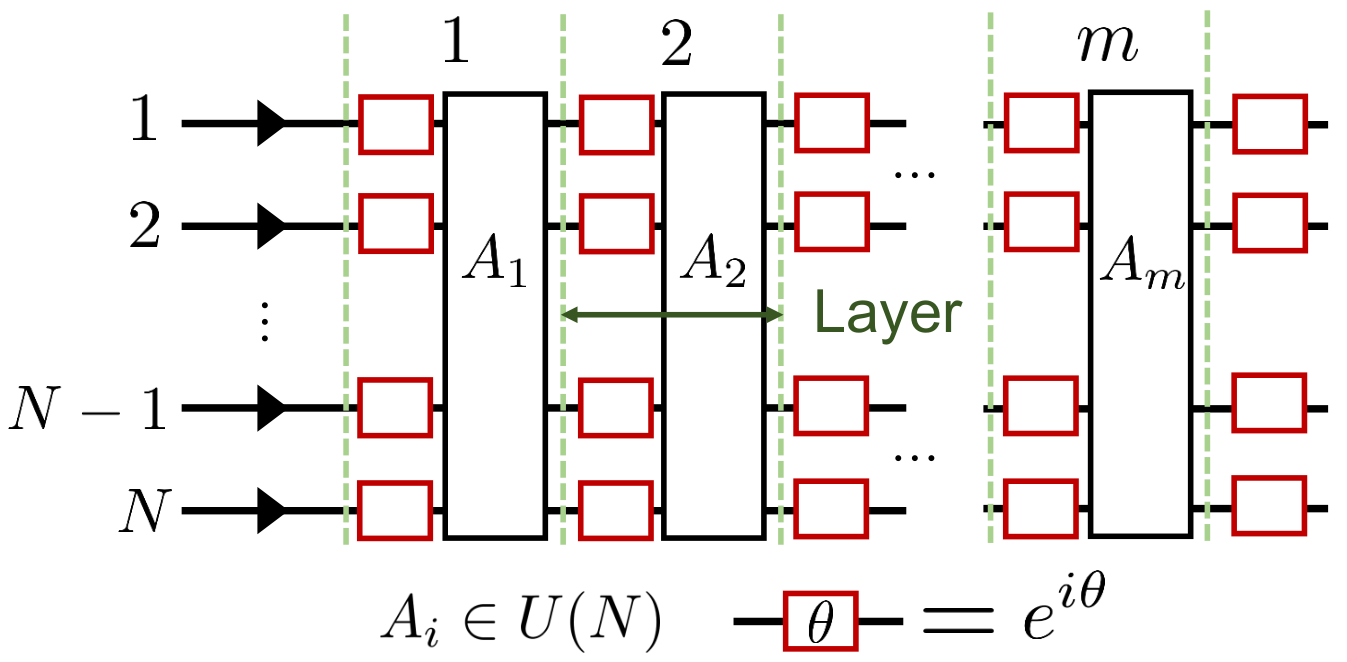
\includegraphics[width=4.5cm]{MPLC.png}
  \vspace{0.6cm}
\end{minipage}
\begin{minipage}[b]{0.31\linewidth}
  \centering
  (b)
  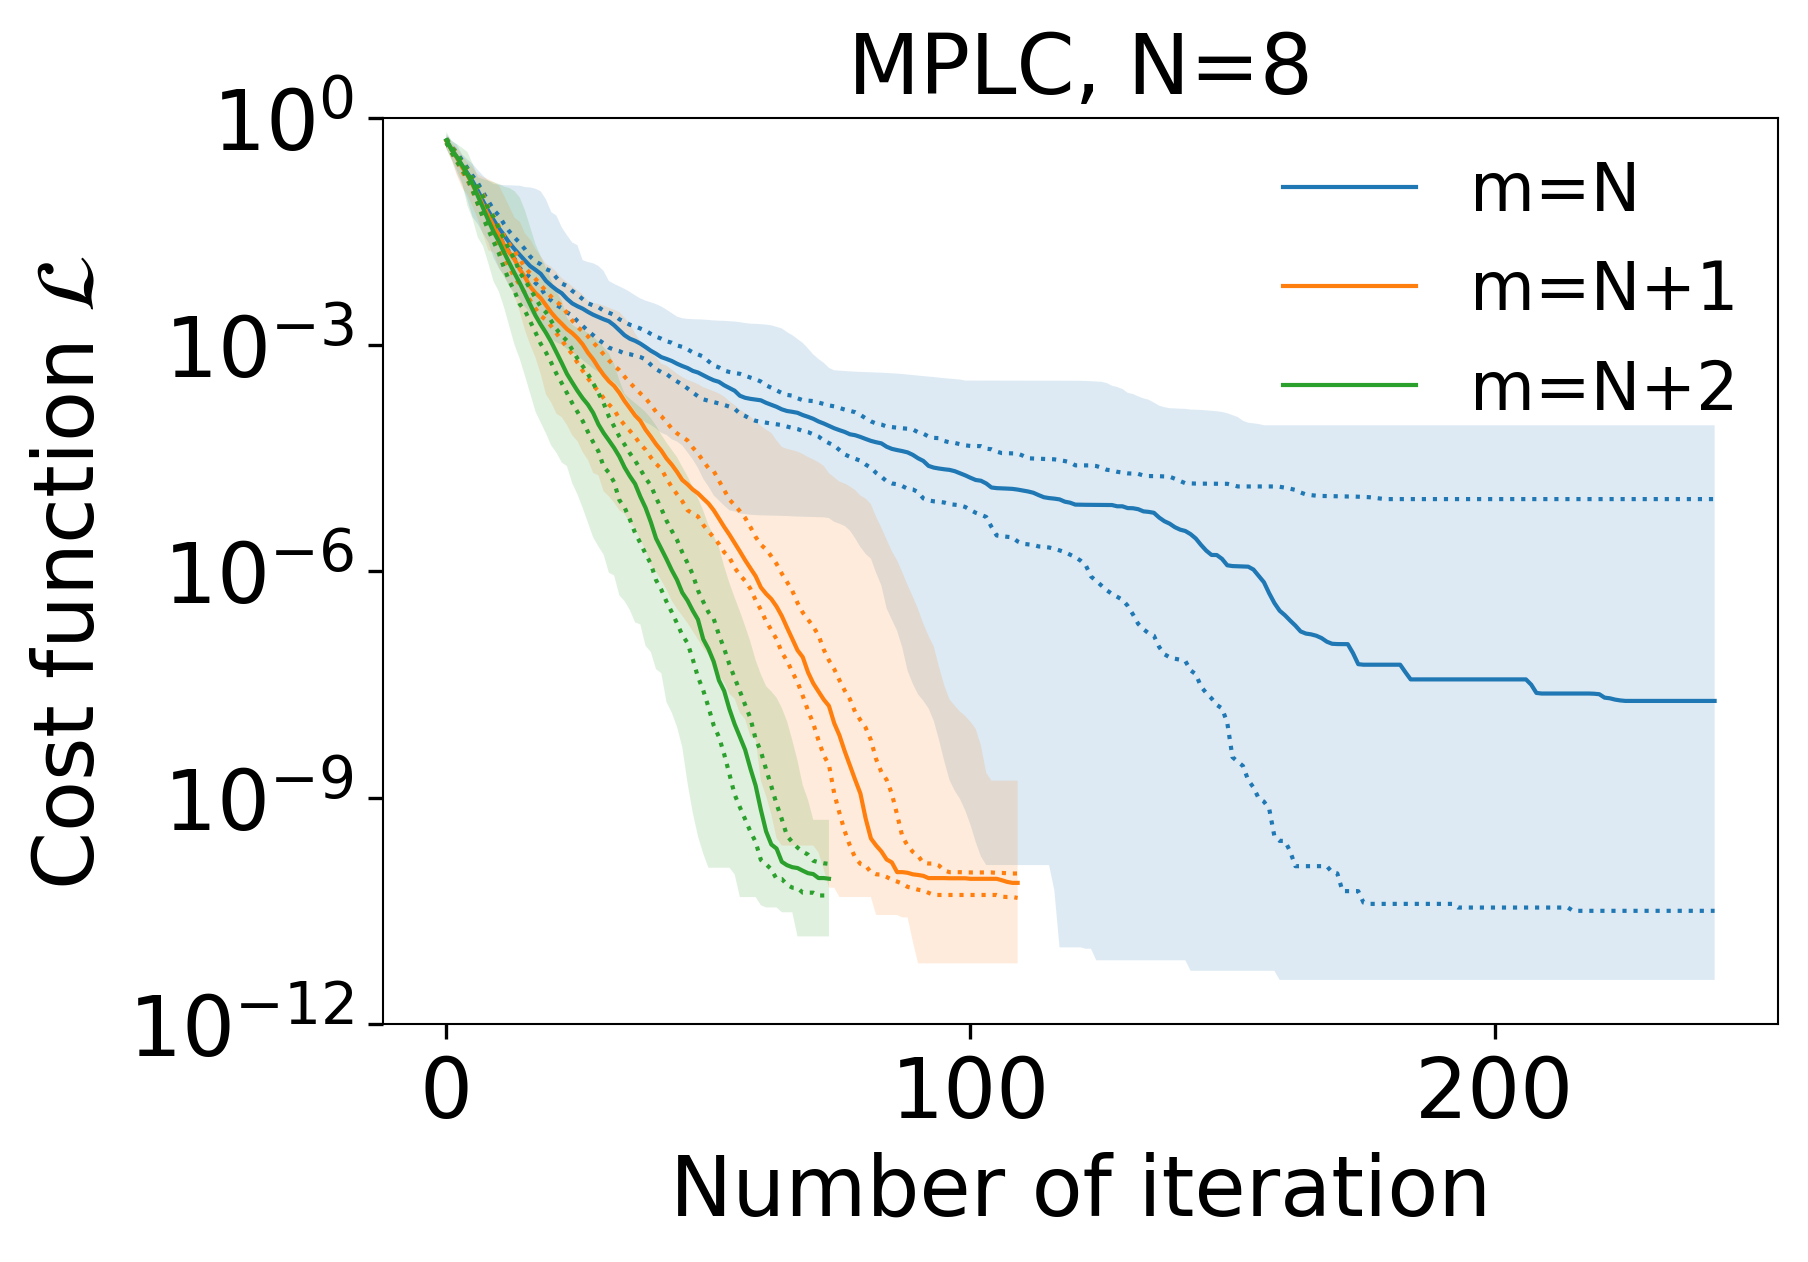
\includegraphics[width=4.4cm]{MPLC_N8.png}
\end{minipage}
\begin{minipage}[b]{0.31\linewidth}
  \centering
  (c)
  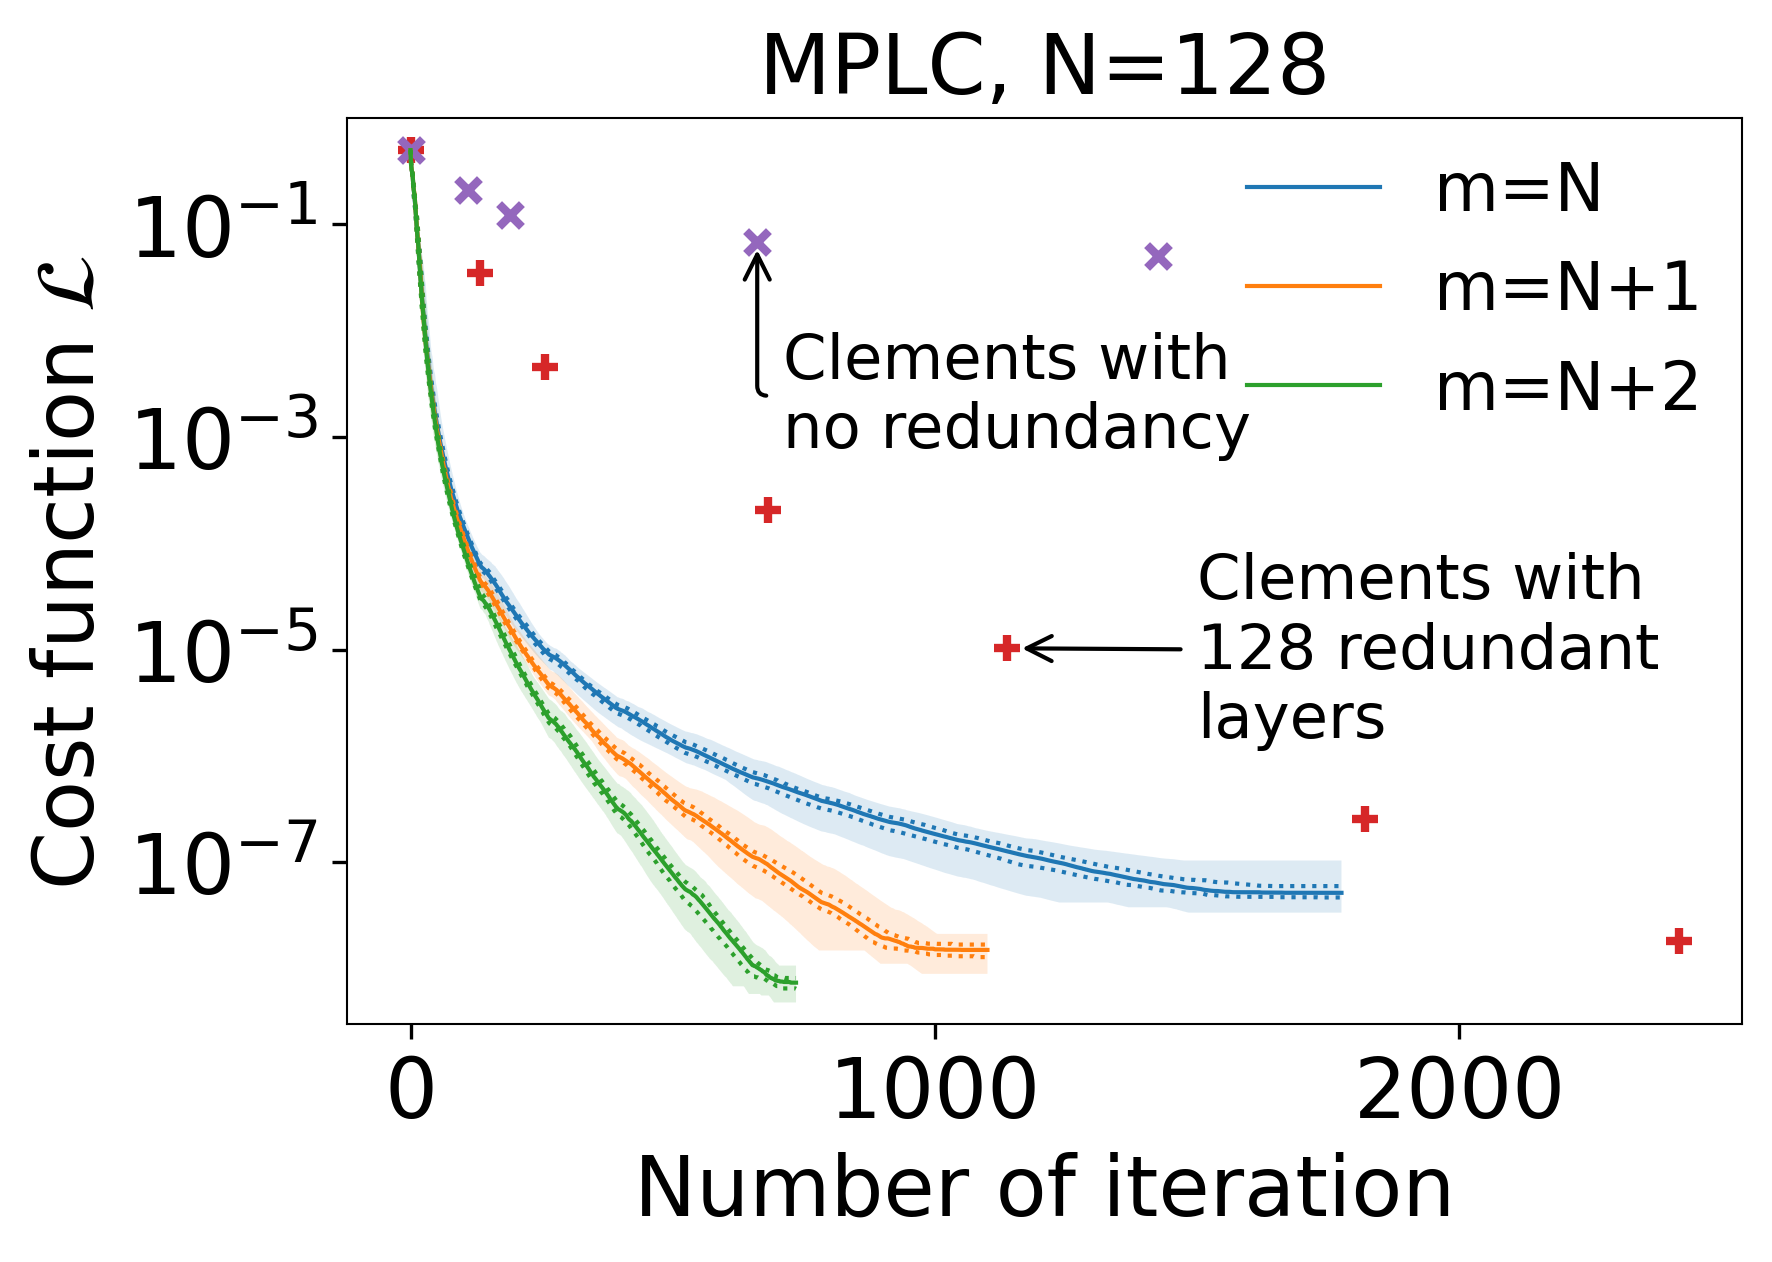
\includegraphics[width=4.4cm]{comparison.png}
\end{minipage}
%prepage a file figure.png, figure.jpg or figure.pdf to use the following command:
%\includegraphics[width=15cm]{figure}
\noindent\footnotesize\textbf{Fig. 1}
  Schematics and convergence plots. (a) MPLC architecture for $N$ ports with $m$ layers. (b) Convergence plots for $N=8$. (c) Comparison with previous study for $N=128$.
\end{quotation}

\setlength\parindent{0pt}\vspace{0ex}
\textbf{Reference}

\footnotesize
[1] W. R. Clements, P. C. Humphreys, B. J. Metcalf, W. S. Kolthammer, and I. A. Walmsley, Optimal design for universal multiport interferometers, Optica \textbf{3}, 1460 (2016).

[2] J.-F. Morizur, L. Nicholls, P. Jian, S. Armstrong, N. Treps, B. Hage, M. Hsu, W. Bowen, J. Janousek, and H.-A. Bachor, Programmable unitary spatial mode manipulation, J. Opt. Soc. Am. A \textbf{27}, 2524 (2010).

[3] S. Pai, B. Bartlett, O. Solgaard, and D. A. B. Miller, Matrix optimization on universal unitary photonic devices, Phys. Rev. Applied \textbf{11}, 064044 (2019).
%[1] J. Itatani, D. Zeidler, J. Levesque, D. M. Villeneuve, and P. B. Corkum, ``Controlling High Harmonic Generation with Molecular Wave Packets,'' Phys. Rev. Lett. \textbf{94}, 123902 (2005).
%For journal articles, authors are listed first, followed by the article’s full title in quotes, the journal’s title abbreviation, the volume number in bold, page number, and the year in parentheses.

\end{document}
